\documentclass{beamer}
\usepackage{epstopdf}
\usepackage{adjustbox}
\usepackage{tikz}
\usepackage{arydshln} %Dotted lines for tables \hdashline \cdashline
%\usepackage{import}
\usepackage[backend=bibtex]{biblatex} % Bibliographies
%\bibliography{beat_bibliography.bib}
\addbibresource{Presentation_Resources/beat_bibliography.bib}
\usetikzlibrary{
	positioning				% Allows 5px above/below of x style positioning
	, arrows				% Allows <-, ->, <-> style arrows.
	, fit					% Allows fitting lines to shapes
	, decorations.pathreplacing	% Allows decoration that affect line paths.
	, backgrounds
	, shapes
	, shapes.multipart
	, calc
	, chains
}
\usepackage{todonotes}

\mode<presentation> {
	\usetheme{Malmoe}
	\usecolortheme{whale}
	\setbeamertemplate{footline}[page number]
	\setbeamertemplate{navigation symbols}{}
}

%----------------------------------------------------------------------------------------
%	TITLE PAGE
%----------------------------------------------------------------------------------------

\title[Short title]{Project NUClear}

\author{
	Trent Houliston \and Jake Woods \and Joshua Kearns \and Michael Burton
}

\institute[UoN]
{
	University of Newcastle \\ % Your institution for the title page
	\medskip
	\textit{\{Trent.Houliston, Jake.F.Woods, Joshua.Kearns, Michael Burton\}@uon.edu.au} % Email address
}

\date{\today}

% Start of document
\begin{document}

%----------------------------------------------------------------------------------------
% Title Slide
%----------------------------------------------------------------------------------------
\begin{frame} % Introduce the team on this slide
	\titlepage % Print the title page as the first slide
\end{frame}


%----------------------------------------------------------------------------------------
\section{Introduction}
%----------------------------------------------------------------------------------------
\begin{frame}
	\frametitle{Introduction to NUbots}
	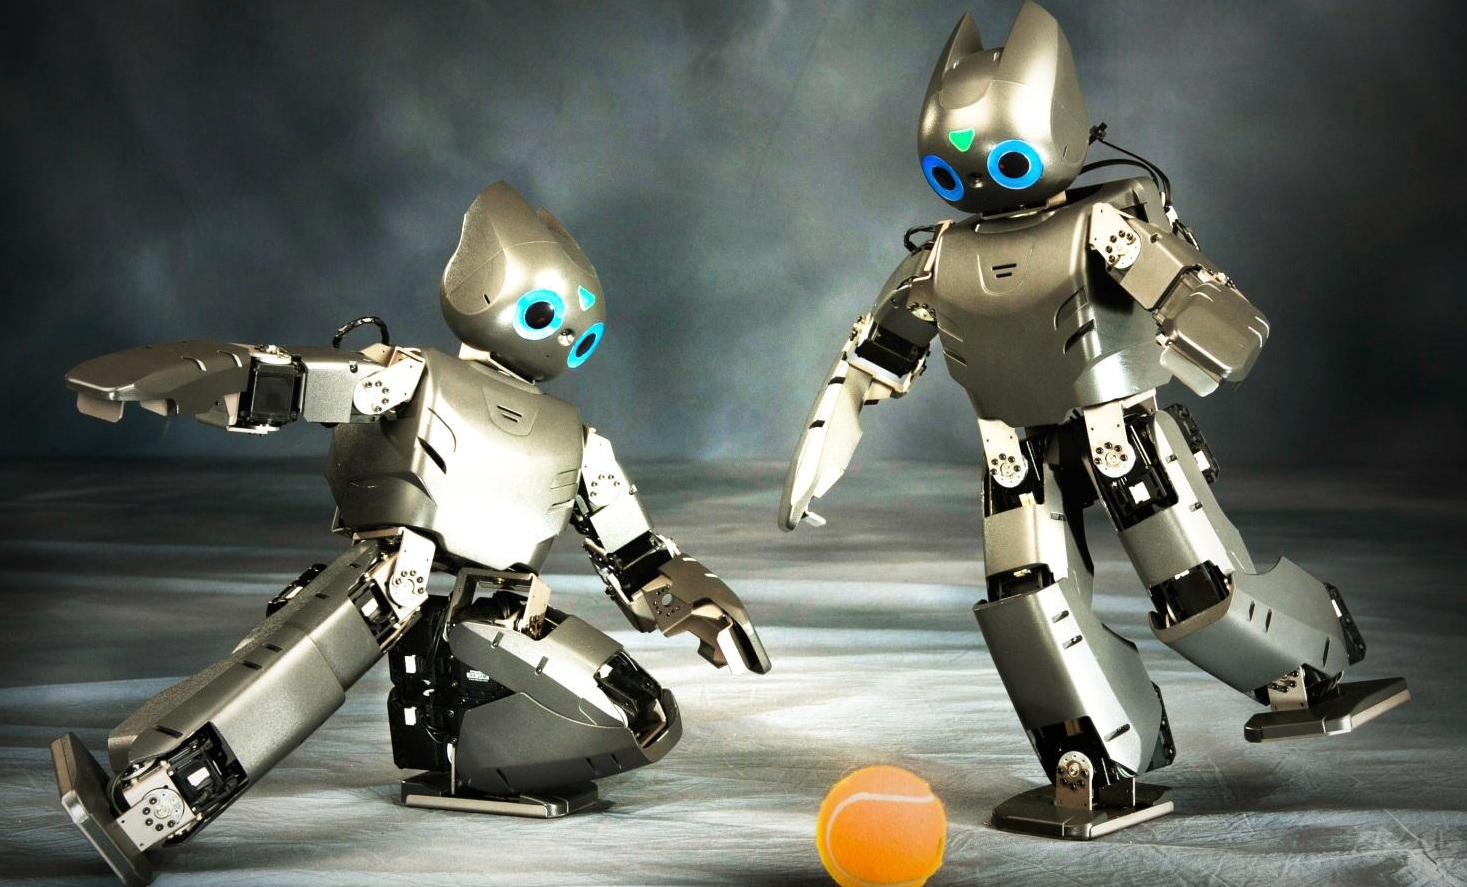
\includegraphics[scale=.25]{Presentation_Images/darwin.jpg}
\end{frame}

\begin{frame}
	\frametitle{Goals}
	\begin{itemize}
		\item Facilitate the use of robots for research, marketing, other non-soccer based behaviours.
		\item Make it easier to take full advantage of the robots hardware.
		\item Improve the time it takes to become effective with the NUbots code.
	\end{itemize}
\end{frame}

\begin{frame}
	\frametitle{Difficulty}
	\begin{itemize}
		\item Estimated cost of \$200,000-\$500,000 (using COCOMO)
		\item Working with C++
		\item Working directly with hardware
		\item Legacy codebase with 182,000 lines of code.
	\end{itemize}
\end{frame}

\begin{frame}
	\frametitle{Successes}
	\begin{itemize}
		\item Worked closely with the NUbots team to ensure the project solves real problems.
		\item Already being used in NUbots research.
	\end{itemize}
\end{frame}

%----------------------------------------------------------------------------------------
\section{Existing System}
%----------------------------------------------------------------------------------------
\begin{frame}
	\sectionpage
\end{frame}

\begin{frame}
	\frametitle{Existing Architecture - Dependency Graph}
	\begin{adjustbox}{max totalsize={\textwidth}{.9\textheight},center}
	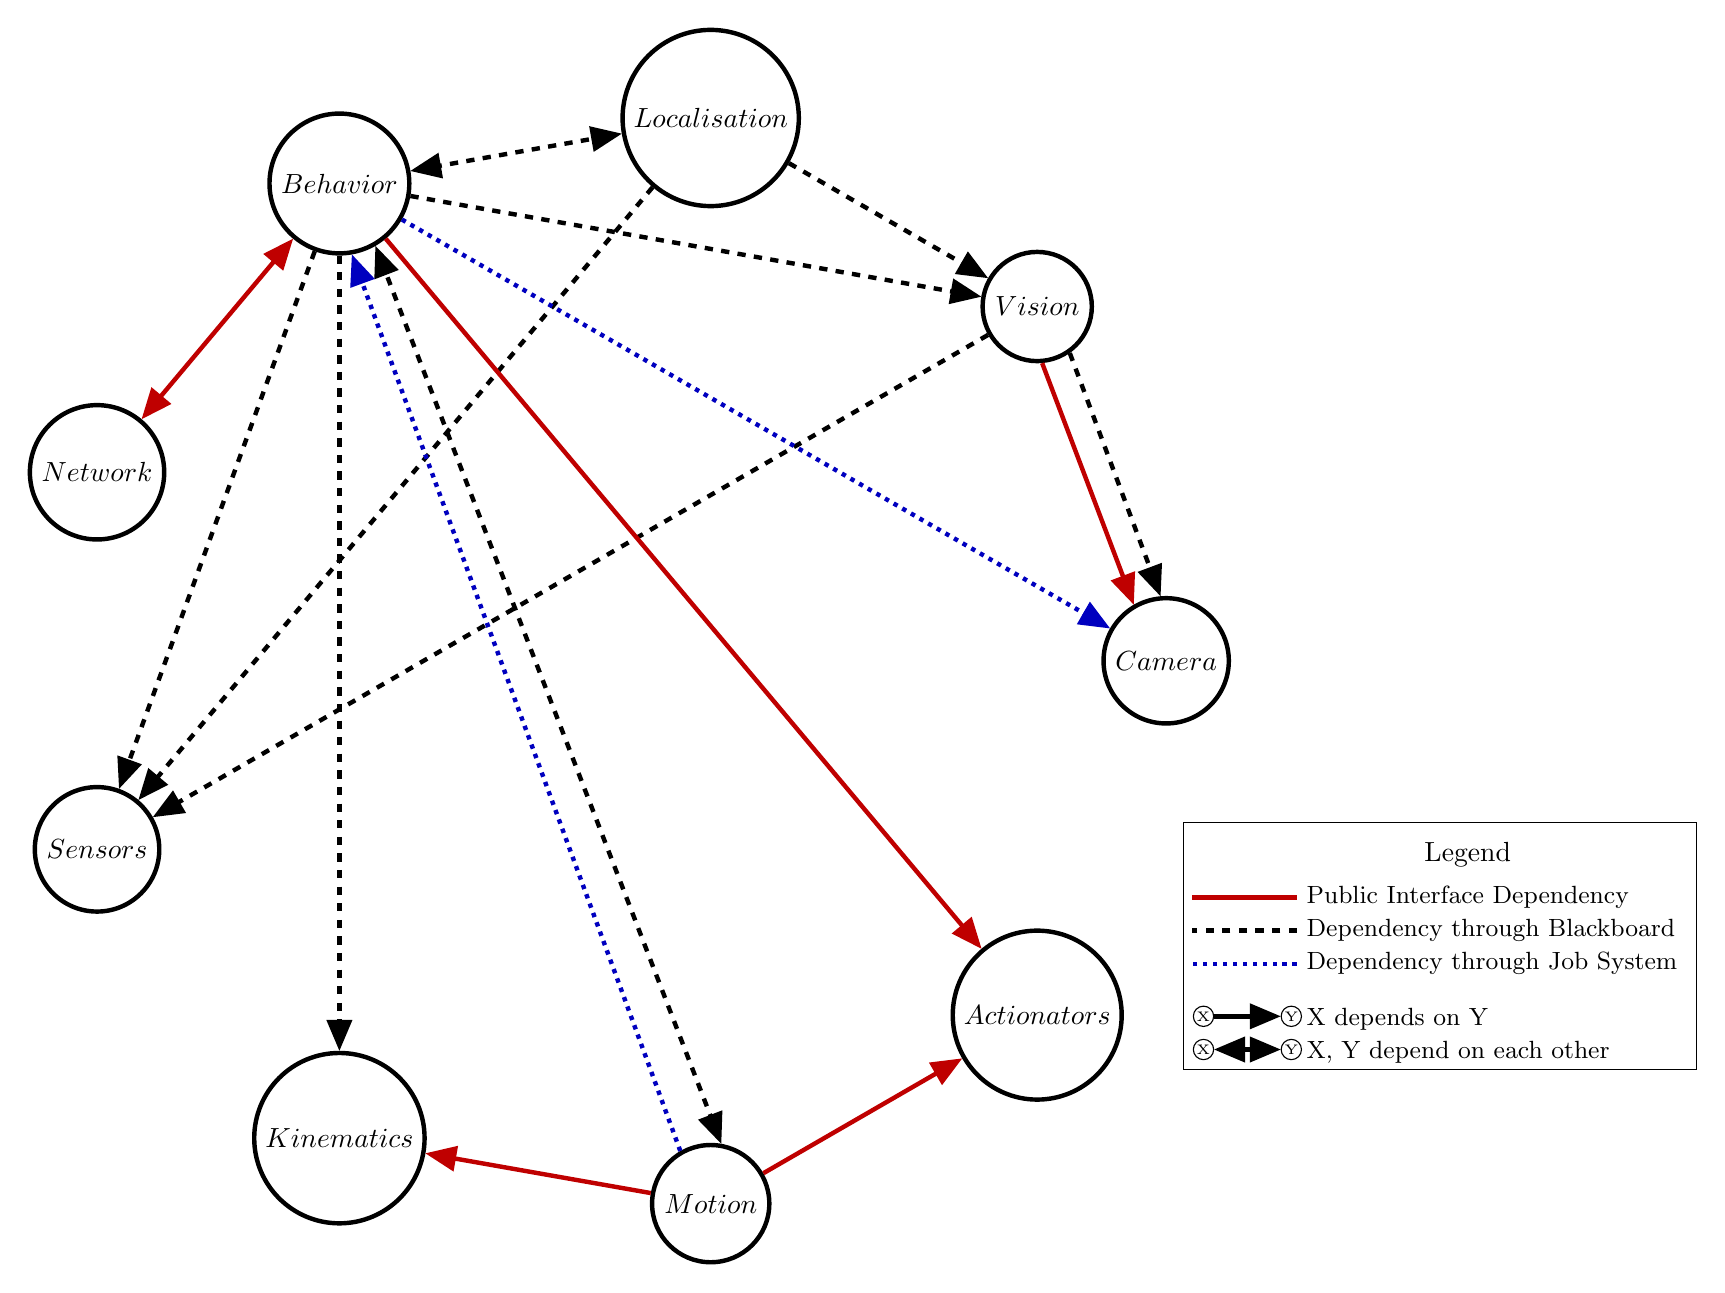
\begin{tikzpicture}[
		reactor/.style={draw, circle, ultra thick}
		, basearrow/.style={>=triangle 45, ultra thick}
		, blackboard/.style={basearrow, dashed}
		, publicinterface/.style={basearrow, color=red!75!black}
		, jobs/.style={basearrow, dotted, color=blue!75!black}
		, dependent/.style={->}
		, codependent/.style={<->}]

		%%% Legend
		\coordinate (legendpoint) at (13, -2);

		%% Public Interface Dependency
		\node [below=of legendpoint,anchor=east] (publicinterfacelabel) {\small Public Interface Dependency};
		\draw [publicinterface] (publicinterfacelabel.mid west) -- ++(-38pt, 0pt);

		%% Blackboard Dependency
		\node [below=12pt of publicinterfacelabel.south west,anchor=south west] (blackboardlabel) {\small Dependency through Blackboard};
		\draw[blackboard] (blackboardlabel.mid west) -- ++(-38pt, 0pt);

		%% Jobs Dependency
		\node [below=12pt of blackboardlabel.south west,anchor=south west] (joblabel) {\small Dependency through Job System};
		\draw[jobs] (joblabel.mid west) -- ++(-38pt, 0pt);

		%% Dependancy Type: Depends on
		\node[below=20pt of joblabel.south west,anchor=south west] (dependencylabel) {\small X depends on Y};
		\node[circle, draw, inner sep=0.5pt] (dependencynodeY) at ([yshift=1pt,xshift=-2pt]dependencylabel.mid west) {\tiny Y};
		\node[circle, draw, inner sep=0.5pt, left=24pt of dependencynodeY] (dependencynodeX) {\tiny X};
		\draw[basearrow, dependent] (dependencynodeX) edge (dependencynodeY);

		%% Dependancy Type: Codependent
		\node[below=12pt of dependencylabel.south west,anchor=south west] (codependencylabel) {\small X, Y depend on each other};
		\node[circle, draw, inner sep=0.5pt] (codependencynodeY) at ([yshift=1pt,xshift=-2pt]codependencylabel.mid west) {\tiny Y};
		\node[circle, draw, inner sep=0.5pt, left=24pt of codependencynodeY] (codependencynodeX) {\tiny X};
		\draw[basearrow, codependent] (codependencynodeX) edge (codependencynodeY);

		%% Legend Header
		\node[above=0pt of publicinterfacelabel] (legendheader) {Legend};

		%%% Draw all of our components in a circle
		\foreach [count=\i] \reactor in {Camera, Vision, Localisation, Behavior, Network, Sensors, Kinematics, Motion, Actionators} {

			% Draw the reactors around the central star
			\node[reactor] (\reactor) at ({360/9 * (\i - 1)}:7cm) {$\reactor$};
		};

		%% Legend Border
		\node[fit=(legendheader)(publicinterfacelabel)(blackboardlabel)
				(joblabel)(dependencylabel)(codependencynodeX)(codependencynodeY),rectangle,draw](legendgroup){};

		%%% Dependencies
		%% Vision
		\path[blackboard, dependent] (Vision.305) edge (Camera.95);
		\path[publicinterface, dependent] (Vision.275) edge (Camera.120);
		\path[blackboard, dependent] (Vision) edge (Sensors);

		%% Localisation
		\path[blackboard, dependent] (Localisation) edge (Sensors);
		\path[blackboard, dependent] (Localisation) edge (Vision);

		%% Behavior
		\path[blackboard, codependent] (Behavior) edge (Localisation);
		\path[blackboard, dependent] (Behavior) edge (Kinematics);
		\path[blackboard, dependent] (Behavior) edge (Vision);
		\path[blackboard, dependent] (Behavior) edge (Sensors);
		\path[publicinterface, dependent] (Behavior) edge (Actionators);
		\path[publicinterface, codependent] (Behavior) edge (Network);
		\path[jobs, dependent] (Behavior) edge (Camera);

		%% Motion
		\path[blackboard, codependent] (Motion.80) edge (Behavior.300);
		\path[jobs, dependent] (Motion.120) edge (Behavior.280);
		\path[publicinterface, dependent] (Motion) edge  (Actionators);
		\path[publicinterface, dependent] (Motion) edge (Kinematics);
	\end{tikzpicture}
	\end{adjustbox}
\end{frame}

\begin{frame}
	\frametitle{Problems in Existing System}
	\begin{itemize}
		\item Heavy Module Dependencies
		\item Tightly Locked to two threads
		\begin{itemize}
			\item Synchronisation Issues cause weird behaviours.
		\end{itemize}
		\item Networking is really hard
		\item Low traceability into execution process
		\item Difficult to automatically test
	\end{itemize}
\end{frame}

%----------------------------------------------------------------------------------------
\section{New Design}
%----------------------------------------------------------------------------------------
\begin{frame}
	\sectionpage
\end{frame}

\subsection{NUClear API}
\begin{frame}
	\frametitle{Software Architecture}
	\begin{itemize}
		\item If we are to replace the architecture of the existing system, we need to define what makes a good architecture
		\item A good software architecture is
		\begin{itemize}
			\item Maintainable
			\item Modifiable
			\item Testable
			\item Understandable
		\end{itemize}
	\end{itemize}
\end{frame}

\begin{frame}
	\frametitle{Coupling and Cohesion}
	\begin{itemize}
		\item The most powerful indicators for good architecture design are those of coupling and cohesion
		\item These two properties have huge influences on how easy a system is to understand and change
		\item A well designed system should be loosely coupled, and tightly cohesive
	\end{itemize}
\end{frame}

\begin{frame}
	\frametitle{Coupling}
	\begin{itemize}
		\item Coupling is a measure of how much a module relies on another module
		\item For example, if a module calls functions on another module, it is dependent on it
		\item A well designed system attempts to minimise these links between modules where possible
		\item It is also important to avoid irrelevant information being communicated
	\end{itemize}
\end{frame}

\begin{frame}
	\frametitle{Cohesion}
	\begin{itemize}
		\item Cohesion is a measure of the extent to which two elements of a single module belong together
		\item It describes the relevance of functionality within a module
		\item For example, if a single module contained only functionality for controlling a robots motion it would be tightly cohesive
		\item However if a single module contained code for both performing vision processing as well as controlling the robots limbs this would be loosely cohesive as the two functions do not belong in a single logical module.
	\end{itemize}
\end{frame}

\begin{frame}
	\frametitle{Coupling}
	\begin{itemize}
		\item From an architectural standpoint, the decision of cohesion must be considered in each module
		\item However coupling must be designed for the entire architecture in order to ensure that communication between modules is loosely coupled
	\end{itemize}
\end{frame}

\begin{frame}
	\frametitle{Levels of Coupling}
	\begin{itemize}
		\item Coupling levels, from most coupled to least coupled are:
		\begin{itemize}
			\item Content Coupling (Pathological Coupling)
			\item Common Coupling (Global Coupling)
			\item External Coupling
			\item Control Coupling
			\item Stamp Coupling
			\item Data Coupling
			\item Message Coupling
			\item No Coupling
		\end{itemize}
		\item The existing architecture uses Common coupling through Blackboard (global storage)
	\end{itemize}
\end{frame}

\begin{frame}
	\frametitle{Message Passing}
	\begin{itemize}
		\item Message passing is a method for components to communicate without explicitly targeting each other
		\item Message coupling is the least coupled method of communication
		\item Message passing systems have excellent maintainability and modifiability
		\item Components require no knowledge of each other
	\end{itemize}
\end{frame}

\begin{frame}
	\frametitle{Existing Systems}
	\begin{itemize}
		\item Message passing systems have been used in robotics before
		\item They have been used in most robotic architectures designed for large scale use
		\item These include
		\begin{itemize}
			\item Robot OS (ROS)
			\item Dynamic Data eXchange (DDX)
			\item CORBA based systems
		\end{itemize}
	\end{itemize}
\end{frame}

\begin{frame}
	\frametitle{Robot OS}
	\begin{itemize}
		\item ROS is of particular note as it is the most commonly used system used in research
		\item It currently runs in many robotic systems and has a substantial array of existing modules for it
		\item It is a message passing system which allows multiple programming languages and machines
	\end{itemize}
\end{frame}

\begin{frame}
	\frametitle{Performance}
	\begin{itemize}
		\item These frameworks are not suitable for use on the NUbots team robots
		\item They were designed to be used on high performance distributed systems
		\item The latency and processing overhead of the message passing is significant on slower systems
		\item This makes them unsuitable for lower performance devices such as the DARwIn-OP platform
	\end{itemize}
\end{frame}

\begin{frame}
	\frametitle{NUClear}
	\begin{itemize}
		\item To resolve these issues a new framework was designed named NUClear
		\item This framework and corresponding architecture is at least one thousand times faster then these systems
		\item This allows its use for the NUbots system
	\end{itemize}
\end{frame}

\begin{frame}
	\frametitle{NUClear Design}
	\centering
	\scalebox{0.55}{
		\begin{tikzpicture}[
				element/.style={
				circle,
				rounded corners,
				draw=black, very thick,
				minimum height=2em,
				text centered
			},
			arrow/.style={
				<->,
				thick
			},
			>=latex]

			\node [element] (plant) {PowerPlant};

			%%% Draw all of our components in a circle
			\foreach [count=\i] \reactor in {Reactor, Reactor, Reactor, Reactor, Reactor} {
				% Draw the reactors around the central star
				\node [element] (reactor) at ({360/5 * (\i)}:6cm) {$\reactor$};

				\path [arrow] (plant) edge (reactor);
			};

		\end{tikzpicture}
	}
\end{frame}

\begin{frame}
	\frametitle{NUClear Design}
	\begin{itemize}
		\item NUClear is designed around a central PowerPlant
		\item The PowerPlant has several ``Reactors'' around it
		\item These reactors request data they need, and emit data they have created to it
		\item The PowerPlant will route this information to the appropriate entities
		\item The PowerPlant is also responsible for the storage of information
	\end{itemize}
\end{frame}

\begin{frame}
	\frametitle{NUClear Design}
	\begin{itemize}
		\item NUClear itself is built around a simple but powerful API
		\item It uses advanced C++ techniques in order to allow an intuitive description of data flow
		\item This allows it to be taught and used by novice C++ users while enforcing good practice
	\end{itemize}
\end{frame}

\begin{frame}
	\frametitle{NUClear Features}
	\begin{itemize}
		\item There have been several features integrated into NUClear which distinguish it as exceptional
		\item These include the following areas
		\begin{itemize}
			\item Transparent Multithreading
			\item Debugging Tools
			\item Integrated Networking
			\item Extensible API
		\end{itemize}
	\end{itemize}
\end{frame}

\begin{frame}
	\frametitle{Transparent Multithreading}
	\begin{itemize}
		\item NUClear is a multithreaded framework
		\item It will transparently multithread any code that is given to it
		\item This allows it to make use of all of the resources in the system
		\item This is also a significant advancement as it makes the system scaleable to future hardware
	\end{itemize}
\end{frame}

\begin{frame}
	\frametitle {Multi Threading}
	\begin{adjustbox}{max totalsize={\textwidth}{\textheight},center}
		\centering
		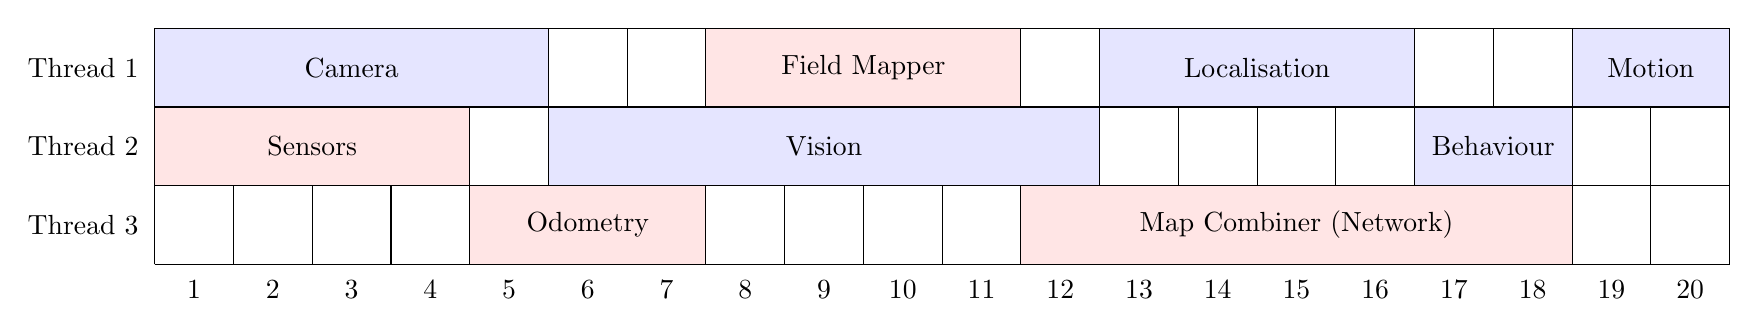
\begin{tikzpicture}
			\begin{scope}[
				task/.style={draw=black},
				cameratriggered/.style={fill=blue!10},
				sensortriggered/.style={fill=red!10}]

				\draw (1, 1) grid (21, 4);

				%% Thread 1
				\draw[cameratriggered, task] (1, 3) rectangle node {Camera} (6, 4);
				\draw[sensortriggered, task] (8, 3) rectangle node {Field Mapper} (12, 4);
				\draw[cameratriggered, task] (13, 3) rectangle node {Localisation} (17, 4);
				\draw[cameratriggered, task] (19, 3) rectangle node {Motion} (21, 4);

				%% Thread 2
				\draw[sensortriggered, task] (1, 2) rectangle node {Sensors} (5, 3);
				\draw[cameratriggered, task] (6, 2) rectangle node {Vision} (13, 3);
				\draw[cameratriggered, task] (17, 2) rectangle node {Behaviour} (19, 3);

				%% Thread 3
				\draw[sensortriggered, task] (5, 1) rectangle node {Odometry} (8, 2);
				\draw[sensortriggered, task] (12, 1) rectangle node {Map Combiner (Network)} (19, 2);

				% Row labels
				\node[anchor=east, inner sep=0] at (.8, 3.5) {Thread 1};
				\node[anchor=east, inner sep=0] at (.8, 2.5) {Thread 2};
				\node[anchor=east, inner sep=0] at (.8, 1.5) {Thread 3};

				% Column Labels
				\foreach \i in {1,...,20} {
				\node[anchor=north, inner sep=0] at (\i + .5, .8) {\i};
				}
			\end{scope}
		\end{tikzpicture}
	\end{adjustbox}
\end{frame}

\begin{frame}
	\frametitle{Debugging Tools}
	\begin{itemize}
		\item Built into NUClear are several debugging and trace tools
		\item Every message that is sent can be tracked and the messages it causes can be identified
		\item We can build a tree of the execution along with how long process executed for
		\item It also captures information such as errors that occur, and even the messages themselves
		\item This allows us to inspect in fine detail the ordering and results of any part of the system
	\end{itemize}
\end{frame}

\begin{frame}
	\frametitle{Integrated Networking}
	\begin{itemize}
		\item The networking system in NUClear is transparent to those using the system
		\item Any data can be sent over the network with no modification
		\item The syntax for emitting data over the network is identical to sending it to other modules
		\item This makes it trivial to perform network communication with other systems
	\end{itemize}
\end{frame}

\begin{frame}
	\frametitle{Extensible API}
	\begin{itemize}
		\item The NUClear API itself was designed to be extensible
		\item The API which is defined in NUClear can be extended by the user
		\item This gives a lot of power to implement features within the language itself
		\item For example, the networking in NUClear is implemented using the extension system
		\item This is useful as networking has system wide influence, integrating it into the API allows a more intuitive codebase
	\end{itemize}
\end{frame}

%----------------------------------------------------------------------------------------
\subsection{NUClear Port}
%----------------------------------------------------------------------------------------
\begin{frame}
	\frametitle{NUClear Port}

	\begin{itemize}
		\item The NUbots software has been ported to use the NUClear architecture
		\item Functionality has been divided into many small, cohesive modules
		\item All communication across modules is accomplished through NUClear messages
		\item A new, flexible build system has been created with `roles' to allow fast and easy adding of functionality
	\end{itemize}
\end{frame}

\begin{frame}
	\frametitle{Modules}

	\begin{itemize}
		\item Every module has a single clear purpose, for example
		\begin{itemize}
			\item interacting with robot hardware
			\item running scripted movements
			\item loading configuration files
		\end{itemize}
		\item Modules do not care which other modules are present, only what information they consume and what they can produce
		\begin{itemize}
			\item Modules with the same inputs and outputs are interchangeable
			\item Platform details are inherently decoupled from everything else
		\end{itemize}
	\end{itemize}
\end{frame}

\begin{frame}
	\frametitle{Testing}

	\begin{itemize}
		\item Testing is built into the new system from the ground up
		\item Every module can have associated unit tests
		\item The build system can run unit tests as a batch
		\item It is easy to test single modules or subsets in isolation
		\item Can create testing modules that emulate input from hardware
	\end{itemize}
\end{frame}

\begin{frame}
	\frametitle{Orchestration}
	\begin{itemize}
		\item Thanks to modular design we can take inspiration from Service Oriented Architecture design
		\item Orchestration is the process of taking several modules and combining them to form an application
		\item The new build system uses `roles' to build behaviours from orchestrated modules
		\begin{itemize}
			\item Robocup role with soccer modules
			\item Marketing role for showing off the robots
			\item Script Tuner role with an interface for tweaking motion scripts
		\end{itemize}
		\item Many modules are shared by multiple roles
	\end{itemize}
\end{frame}

\begin{frame}
	\frametitle{Existing vs. New}

	\begin{itemize}
		\item In the existing system
		\begin{itemize}
			\item Inducting a new member into the project takes one month
			\item Changing behaviour requires detailed understanding, lots of code changes
		\end{itemize}
		\item In the NUClear port
		\begin{itemize}
			\item Modules are easy to learn and don't require understanding all their dependencies
			\item A new member can start doing useful work almost immediately
			\item Creating new roles requires changing only one file
		\end{itemize}
		\item `Mechwarrior' was created in under an hour on the new system, ``would have been impossible'' on the existing system
	\end{itemize}
\end{frame}

\begin{frame}
	\huge MechWarrior Demonstration
\end{frame}

%----------------------------------------------------------------------------------------
\section{Robot Dance}
%----------------------------------------------------------------------------------------
	\begin{frame}
		\sectionpage %Title page for the Robot Dance section
	\end{frame}
	\subsection{What and Why?} %-------------------
	\begin{frame}
		\frametitle{Robot Dance: What and Why?}
		\begin{itemize}
			\item Why Dancing Robots?
			\begin{itemize}
				\item Demonstrates the efficiency of the new architecture
				\item Useful for marketing
			\end{itemize}
			\item What does you mean by dancing robots?
			\begin{itemize}
				\item Scripted dancing
				\item Dancing in time with music
			\end{itemize}
		\end{itemize}
	\end{frame}
	\subsection{Dancing to Music} %-------------------
	\begin{frame}
		\frametitle{Dancing to Music}
		\begin{itemize}
			\item Music detected through Microphone
			\item Music analysed to find beats
			\item Dance move chosen and scaled to be in time with latest beats
			\item Dance move is enacted
		\end{itemize}
	\end{frame}
	\subsection{Dancing and NUClear} %-------------------
	\begin{frame}
		\frametitle{Dancing and the New Architecture}
		\framesubtitle{Dancing to a Music}
		\begin{figure}
			\centering
			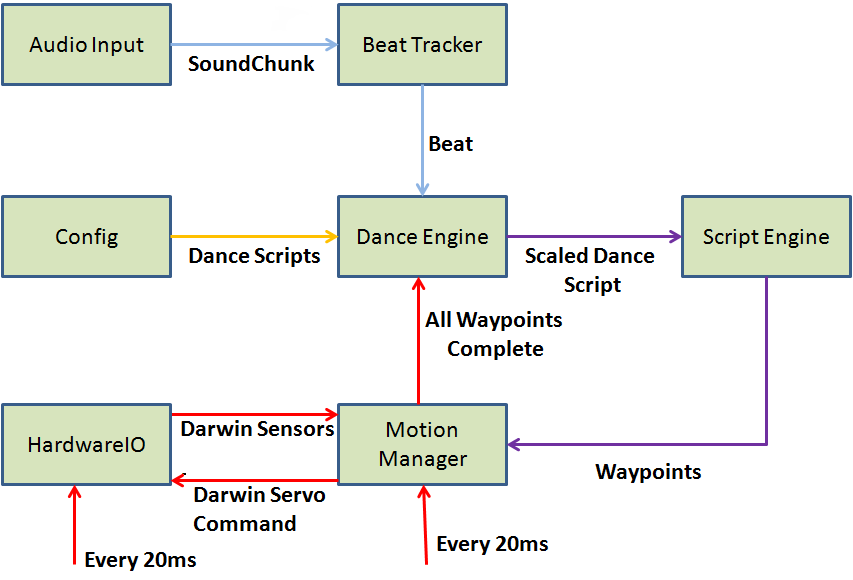
\includegraphics[scale=.45]{Presentation_Resources/dance_audio_new_arc.png}
			\caption{Components for Dancing to Music with the NUClear}
		\end{figure}
	\end{frame}
	\begin{frame}
		\frametitle{Dancing and the New Architecture}
		\framesubtitle{Dancing to a Music}
		\begin{figure}
			\centering
			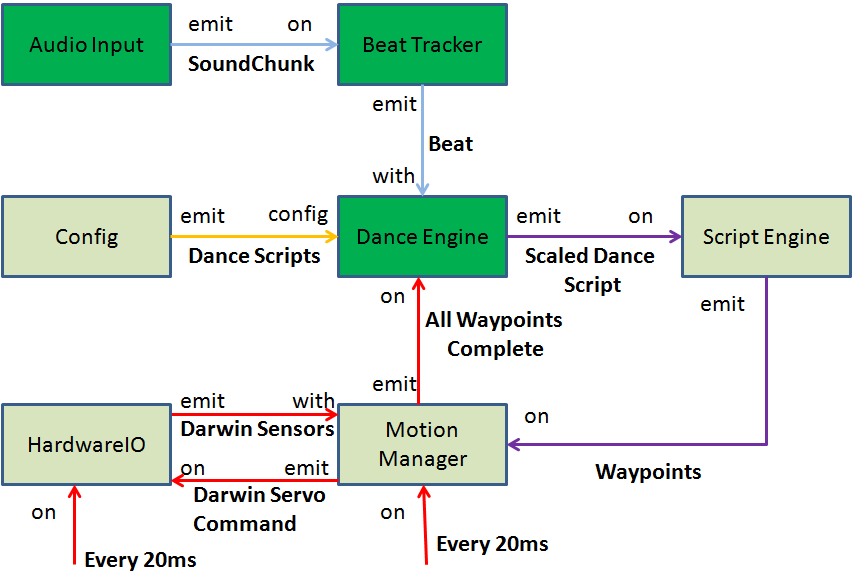
\includegraphics[scale=.45]{Presentation_Resources/dance_audio_new_arc_change.png}
			\caption{Components for Dancing to Music with the NUClear}
		\end{figure}
	\end{frame}
	\subsection{Dancing and the Old Architecture} %-------------------
	\begin{frame}
		\frametitle{Dancing and the Old Architecture}
		\framesubtitle{Dancing to a Music}
		\definecolor{darkGreen}{RGB}{0,176,80}
		\definecolor{lightGreen}{RGB}{146,208,80}
		\definecolor{dullGreen}{RGB}{215,228,189}

		\begin{figure}
			\begin{adjustbox}{max totalsize={\textwidth}{.8\textheight},center}
			\begin{tikzpicture}[
				reactor/.style={draw, circle, ultra thick}
				, basearrow/.style={>=triangle 45, ultra thick}
				, blackboard/.style={basearrow, dashed}
				, publicinterface/.style={basearrow, color=red!75!black}
				, jobs/.style={basearrow, dotted, color=blue!75!black}
				, dependent/.style={->}
				, codependent/.style={<->}
				, new/.style={fill=darkGreen}
				, modified/.style={fill=lightGreen}
				, same/.style={fill=dullGreen}
				, remove/.style={fill=red!50}]

				%%% Legend
				\coordinate (legendpoint) at (14, -2);

				%% Public Interface Dependency
				\node [below=of legendpoint,anchor=east] (publicinterfacelabel) {\small Public Interface Dependency};
				\draw [publicinterface] (publicinterfacelabel.mid west) -- ++(-38pt, 0pt);

				%% Blackboard Dependency
				\node [below=12pt of publicinterfacelabel.south west,anchor=south west] (blackboardlabel) {\small Dependency through Blackboard};
				\draw[blackboard] (blackboardlabel.mid west) -- ++(-38pt, 0pt);

				%% Jobs Dependency
				\node [below=12pt of blackboardlabel.south west,anchor=south west] (joblabel) {\small Dependency through Job System};
				\draw[jobs] (joblabel.mid west) -- ++(-38pt, 0pt);

				%% Dependancy Type: Depends on
				\node[below=20pt of joblabel.south west,anchor=south west] (dependencylabel) {\small X depends on Y};
				\node[circle, draw, inner sep=0.5pt] (dependencynodeY) at ([yshift=1pt,xshift=-2pt]dependencylabel.mid west) {\tiny Y};
				\node[circle, draw, inner sep=0.5pt, left=24pt of dependencynodeY] (dependencynodeX) {\tiny X};
				\draw[basearrow, dependent] (dependencynodeX) edge (dependencynodeY);

				%% Dependancy Type: Codependent
				\node[below=12pt of dependencylabel.south west,anchor=south west] (codependencylabel) {\small X, Y depend on each other};
				\node[circle, draw, inner sep=0.5pt] (codependencynodeY) at ([yshift=1pt,xshift=-2pt]codependencylabel.mid west) {\tiny Y};
				\node[circle, draw, inner sep=0.5pt, left=24pt of codependencynodeY] (codependencynodeX) {\tiny X};
				\draw[basearrow, codependent] (codependencynodeX) edge (codependencynodeY);

				%% Legend Header
				\node[above=0pt of publicinterfacelabel] (legendheader) {Legend};

				%%% Draw all of our components in a circle
				\foreach [count=\i] \reactor/\style in {{Camera/remove}, {Vision/remove}, {Localisation/remove}, {Behavior/modified}, {Network/remove}, {Sensors/same}, {Kinematics/same}, {Motion/modified}, {Actionators/same}, {AudioInput/new}, {BeatTracker/new}} {

					% Draw the reactors around the central star
					\node[reactor, \style] (\reactor) at ({360/11 * (\i - 1)}:7cm) {$\reactor$};
				};

				%% Legend Border
				\node[fit=(legendheader)(publicinterfacelabel)(blackboardlabel)
						(joblabel)(dependencylabel)(codependencynodeX)(codependencynodeY),rectangle,draw](legendgroup){};

				%%% Dependencies
				%% Vision
				\path[blackboard, dependent] (Vision.305) edge (Camera.95);
				\path[publicinterface, dependent] (Vision.275) edge (Camera.120);
				\path[blackboard, dependent] (Vision) edge (Sensors);

				%% Localisation
				\path[blackboard, dependent] (Localisation) edge (Sensors);
				\path[blackboard, dependent] (Localisation) edge (Vision);

				%% Behavior
				\path[blackboard, codependent] (Behavior) edge (Localisation);
				\path[blackboard, dependent] (Behavior) edge (Kinematics);
				\path[blackboard, dependent] (Behavior) edge (Vision);
				\path[blackboard, dependent] (Behavior) edge (Sensors);
				\path[publicinterface, dependent] (Behavior) edge (Actionators);
				\path[publicinterface, codependent] (Behavior) edge (Network);
				\path[jobs, dependent] (Behavior) edge (Camera);

				%% Motion
				\path[blackboard, codependent] (Motion.80) edge (Behavior.300);
				\path[jobs, dependent] (Motion.120) edge (Behavior.280);
				\path[publicinterface, dependent] (Motion) edge  (Actionators);
				\path[publicinterface, dependent] (Motion) edge (Kinematics);

				%% Dance
				\path[blackboard, dependent] (BeatTracker) edge (AudioInput);
				\path[blackboard, dependent] (Behavior) edge (BeatTracker);
			\end{tikzpicture}
			\end{adjustbox}

			%\caption{Components for Dancing to Music with the Old System}
		\end{figure}
	\end{frame}

	\begin{frame}
		\huge Dance Demonstration
	\end{frame}

	\subsection{Conclusion} %-------------------
	\begin{frame}
		\frametitle{Conclusion}
			We achieved our major goals.
			\begin{itemize}
				\item Accepted by the NUbots team as a significant improvement.
				\item Modular Design proven by Dance and MechWarrior
				\item Improvements on some existing low-level code
			\end{itemize}
	\end{frame}

	\begin{frame}
		\huge Questions?
	\end{frame}

%----------------------------------------------------------------------------------------
\section{Individual Research}
%----------------------------------------------------------------------------------------
\begin{frame}
	\sectionpage
\end{frame}

	%----------------------------------------------------------------------------------------
	\subsection{Overcoming Limits of Event Driven Architectures}
	%----------------------------------------------------------------------------------------
	\begin{frame}
		\subsectionpage
	\end{frame}

	\begin{frame}
		\frametitle{What is an event driven architecture?}

		Event Driven Architectures are characterised by a set of modules that communicate using events or messages.
		\begin{itemize}
			\item Events are defined blobs of data with a known format.
			\item \textbf{Event} is often interchangeable with \textbf{Message}
			\item Modules are sometimes be categorised as either \textbf{Producers} or \textbf{Consumers}
		\end{itemize}

	\end{frame}

	\begin{frame}
		\frametitle {Exploring the limits}

		Most event driven architecture limitations can be overcome
		\begin{itemize}
			\item ... given you're willing to sacrifice performance
		\end{itemize}

		The essence of architecture is making decisions
		\begin{itemize}
			\item Performance or Features
			\item Competing choices will change depending on your goal
			\item Different architectures value different things
		\end{itemize}
	\end{frame}

	\begin{frame}
		\frametitle{Common Tradeoffs}

		Message Format
		\begin{itemize}
			\item \textbf{Language-Specific} or \textbf{Language-Agnostic}
			\item \textbf{Human Readable} or \textbf{Machine Only}
		\end{itemize}

		Message Routing
		\begin{itemize}
			\item \textbf{Guaranteed Delivery} or \textbf{Assumed Delivery}
			\item \textbf{Distributed} or \textbf{Central}
			\item \textbf{Inter-Process} or \textbf{In-Process}
		\end{itemize}
	\end{frame}

	\begin{frame}
		\frametitle{Trade Offs: Robot OS and CORBA}
		Goal: Sharing and Collaboration

		Message Format
		\begin{itemize}
			\item \textbf{Language-Agnostic}
			\item \textbf{Human Readable}
		\end{itemize}

		Message Routing
		\begin{itemize}
			\item \textbf{Guaranteed Delivery} and \textbf{Assumed Delivery}
			\item \textbf{Central}
			\item \textbf{Inter-Process}
		\end{itemize}
	\end{frame}

	\begin{frame}
		\frametitle{Trade Offs: NUClear}

		Goal: Speed and Ease-of-Use

		Message Format
		\begin{itemize}
			\item \textbf{Language-Specific} and \textbf{Language-Agnostic}
			\item \textbf{Machine Only}
		\end{itemize}

		Message Routing
		\begin{itemize}
			\item \textbf{Guaranteed Delivery} and \textbf{Assumed Delivery}
			\item \textbf{Distributed}
			\item \textbf{In-Process} and \textbf{Inter-Process}
		\end{itemize}
	\end{frame}

	\begin{frame}
		\frametitle{Use in FYP}

		Using the lessons learned from analysing existing event driven architectures we:
		\begin{itemize}
			\item Decided to keep things primarily In-Process to allow us to provide features with no runtime cost.
			\item Settled on using primarily a Machine-Only and Language-Specific transport only using Language-Agnostic when necessary.
		\end{itemize}
	\end{frame}

	%----------------------------------------------------------------------------------------
	\subsection{Compile Time Message Routing}
	%----------------------------------------------------------------------------------------
	\begin{frame}
		\subsectionpage
	\end{frame}

	\begin{frame}
		\frametitle{Why Messages?}
		\begin{itemize}
			\item As discussed in the main presentation, message passing is slow
			\item If this is the case, why did we go to the trouble of implementing another system
			\item The answer is that in our system, I developed a new technique
		\end{itemize}
	\end{frame}

	\begin{frame}
		\frametitle{Metaprogramming}
		\begin{itemize}
			\item A Metaprogram is a programs that manipulate itself
			\item This includes programs that run at compilation time rather then runtime
			\item It allows work to be offloaded from runtime processing
		\end{itemize}
	\end{frame}

	\begin{frame}
		\frametitle{C++ Template Metaprogramming}
		\begin{itemize}
			\item C++ metaprogramming is done through templates
			\item Templates were designed to implement generic programming
			\item However they also accidentally as a side effect are a turing complete language
			\item This allows programs to be executed using templates at compile time using the type system
		\end{itemize}
	\end{frame}

	\begin{frame}
		\frametitle{Partial Evaluation}
		\begin{itemize}
			\item One such metaprogramming technique is partial evaluation
			\item It applies when partial information is available at compile time
			\item Partial evaluation takes a function and performs part of the evaluation during compilation
			\item In the case of a message passing system the routing of the message is known
		\end{itemize}
	\end{frame}

	\begin{frame}
		\frametitle{Compile Time Message Routing}
		\begin{itemize}
			\item We know the routes messages are going to take at compile time
			\item Messages are published subscribed to using types
			\item We can evaluate the dispatch of these messages at compile time using template metaprograms
			\item We can bind the data of the messages at runtime
		\end{itemize}
	\end{frame}

	\begin{frame}
		\frametitle{Before Compilation}
		\centering
		\scalebox{0.55}{
			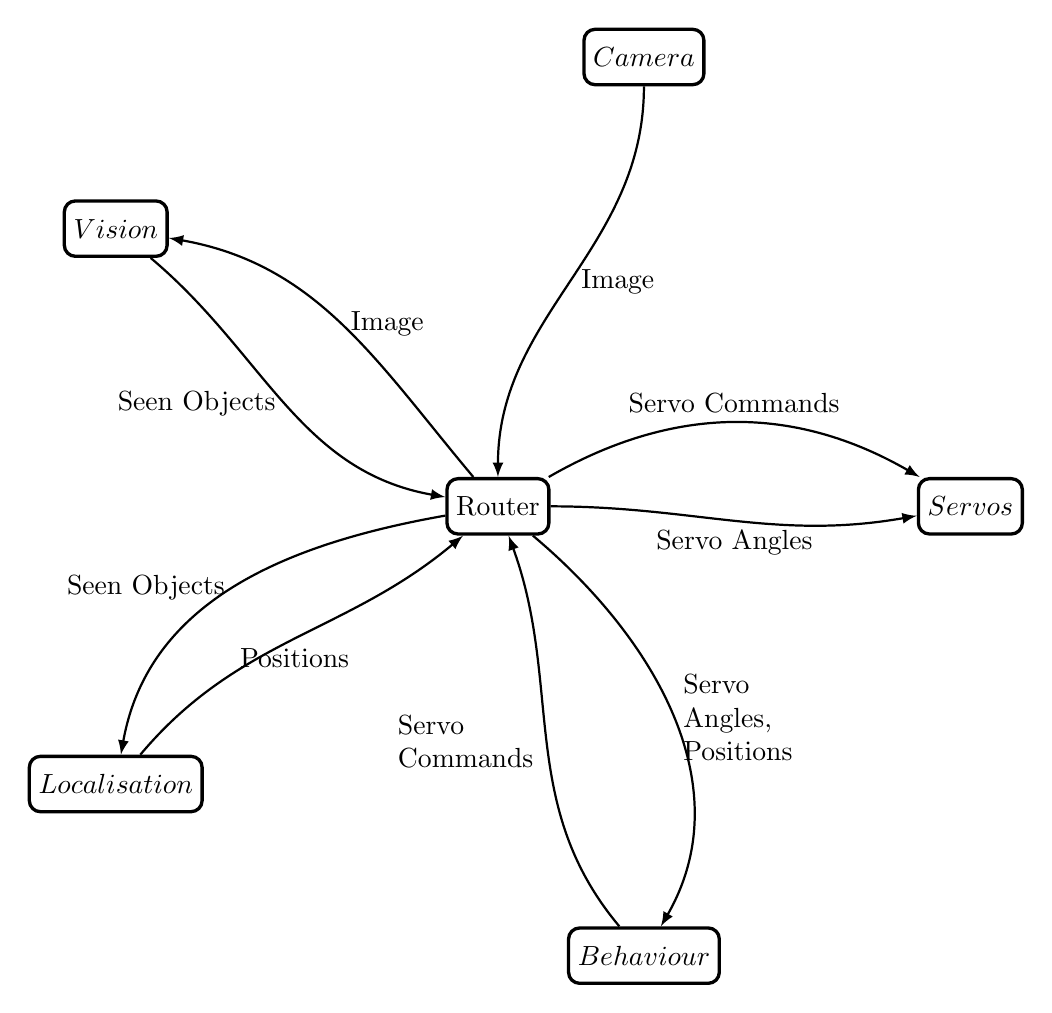
\begin{tikzpicture}[
				element/.style={
				rectangle,
				rounded corners,
				draw=black, very thick,
				minimum height=2em,
				text centered
			},
			ball/.style={
				element,
				minimum height=0,
				fill=black
			},
			arrow/.style={
				->,
				thick
			},
			>=latex]

			\node [element] (router) {Router};

			%%% Draw all of our components in a circle
			\foreach [count=\i] \reactor in {Camera, Vision, Localisation, Behaviour, Servos} {
				% Draw the reactors around the central star
				\node [element] (msg\reactor) at ({360/5 * (\i)}:6cm) {$\reactor$};
			};

			\path [arrow] (router) edge[out=130, in=350]  node[right] {Image} (msgVision);
			\path [arrow] (msgVision) edge[out=320, in=170] node[left] {Seen Objects} (router);

			\path [arrow] (msgCamera) edge[out=270, in=90] node[right] {Image} (router);

			\path [arrow] (router) edge[out=320, in=60] node[right, text width=1.5cm] {Servo Angles, Positions} (msgBehaviour);
			\path [arrow] (msgBehaviour) edge[out=130, in=290] node[left, text width=1.75cm] {Servo Commands} (router);

			\path [arrow] (router) edge[out=190, in=80] node[left] {Seen Objects} (msgLocalisation);
			\path [arrow] (msgLocalisation) edge[out=50, in=220] node[below] {Positions} (router);

			\path [arrow] (router) edge[out=30, in=150] node[above] {Servo Commands} (msgServos);
			\path [arrow] (router) edge[out=0, in=190] node[below] {Servo Angles} (msgServos);

		\end{tikzpicture}}
	\end{frame}

	\begin{frame}
		\frametitle{After Compilation}
		\centering
		\scalebox{0.8}{
			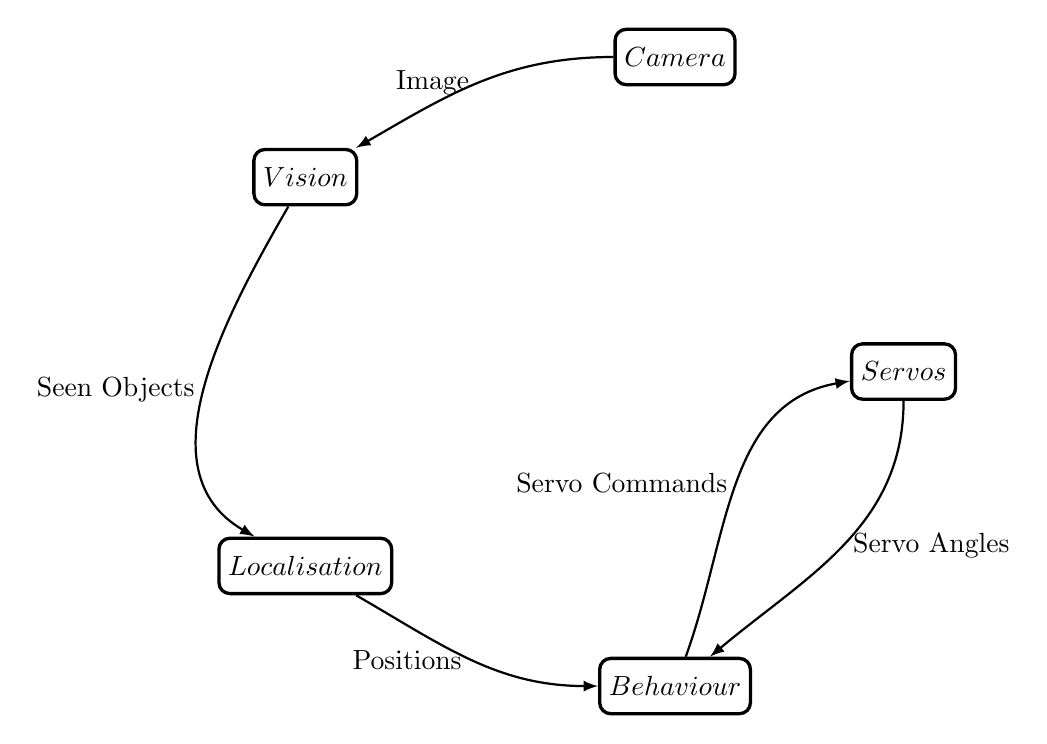
\begin{tikzpicture}[
				scale=0.7,
				element/.style={
					rectangle,
					rounded corners,
					draw=black, very thick,
					minimum height=2em,
					text centered
				},
				ball/.style={
					element,
					minimum height=0,
					fill=black
				},
				arrow/.style={
					->,
					thick
				},
				>=latex]

			%%% Draw all of our components in a circle
			\foreach [count=\i] \reactor in {Camera, Vision, Localisation, Behaviour, Servos} {
				% Draw the reactors around the central star
				\node [element] (comp\reactor) at ({360/5 * (\i)}:6cm) {$\reactor$};
			};

			\path [arrow] (compCamera) edge[out=180, in=30] node[left] {Image} (compVision);
			\path [arrow] (compVision) edge[out=240, in=150] node[left] {Seen Objects} (compLocalisation);
			\path [arrow] (compLocalisation) edge[out=330, in=180] node[left] {Positions} (compBehaviour);
			\path [arrow] (compBehaviour) edge[out=70, in=190] node[left] {Servo Commands} (compServos);
			\path [arrow] (compServos) edge[out=270, in=40] node[right] {Servo Angles} (compBehaviour);

		\end{tikzpicture}}
	\end{frame}

	\begin{frame}
		\frametitle{Compile Time  Message Routing}
		\begin{itemize}
			\item Before compilation, every item only knows about the router
			\item This makes it very simple to modify programs
			\item After compilation components directly access each other
			\item This makes the resulting system almost as fast as direct function access
		\end{itemize}
	\end{frame}

	\begin{frame}
		\frametitle{Compile Time  Message Routing}
		\begin{itemize}
			\item The fast final result from the compile time program allows this architecture to be used
			\item The performance drawbacks of having a message router no longer apply
			\item This allows this style of architecture to be used in performance critical use cases
		\end{itemize}
	\end{frame}

	\begin{frame}
		\frametitle{Type Safety}
		\begin{itemize}
			\item When using message passing with compile time routing there is type safety
			\item This is significant as other message passing systems often have to reinterpret the type
			\item When writing code this provides the advantage of knowing that you are using the correct type
		\end{itemize}
	\end{frame}

	\begin{frame}
		\frametitle{Drawbacks}
		\begin{itemize}
			\item Using compile time message routing has drawbacks
			\item As the routing is performed at compile time, compilation of programs is slower
			\item Also, as template meta-programming in c++ is complex this makes it difficult to use
			\item It also results in larger binaries as the routes for messages are hard coded
			\item The system also requires an optimising compiler, else the system ends slower then a typical function call
		\end{itemize}
	\end{frame}

	\begin{frame}
		\frametitle{Results}
		\begin{itemize}
			\item When compared other methods of message passing compile time routing performed orders of magnitude faster
			\item As routing is performed at compile time, it also does not suffer from a slowdown as the number of publishers, subscribers, or message types increases
			\item The system was compared to CORBA for latency
			\item Compile time dispatch was measured as taking from the range of 300 nanoseconds to 1 microsecond
			\item CORBA is measured as taking between 1 millisecond to 7 milliseconds
		\end{itemize}
	\end{frame}

	\begin{frame}
		\frametitle{Use in FYP}
		\begin{itemize}
			\item Compile time message routing is used within the NUClear framework in order to route messages
			\item This allows it to perform orders of magnitude faster then competing architectures
			\item It also does not suffer slowdowns with the size of the project
		\end{itemize}
	\end{frame}

	\begin{frame}
		\frametitle{Conclusions}
		\begin{itemize}
			\item Compile time dispatch allows message passing to be very fast
			\item We gain the advantages of loose coupling
			\item We also gain the speed that comes from tight coupling
		\end{itemize}
	\end{frame}

	\begin{frame}
		\huge Questions?
	\end{frame}

	\begin{frame}
		\frametitle{References}
		\begin{itemize}
			\item Todd L Veldhuizen. C++ templates as partial evaluation. arXiv preprint cs/9810010, 1998.	\item Timothy H Harrison, David L Levine, and Douglas C Schmidt. The de- sign and performance of a real-time corba event service. ACM SIGPLAN Notices, 32(10):184–200, 1997.
			\item Christopher D Gill, David L Levine, and Douglas C Schmidt. The design and performance of a real-time corba scheduling service. In Challenges in Design and Implementation of Middlewares for Real-Time Systems, pages 3–40. Springer, 2001.
		\end{itemize}
	\end{frame}

	%----------------------------------------------------------------------------------------
	\subsection{Efficient Multithreading in Message Passing Systems}
	%----------------------------------------------------------------------------------------
	\begin{frame}
		\subsectionpage
	\end{frame}

	\begin{frame}
		\frametitle{Challenges of Multithreading}

		\begin{itemize}
			\item It is difficult to divide a complex process into independent blocks that can run in parallel
			\item Some components depend on others' output
			\item Access to shared resources must be synchronised
		\end{itemize}
	\end{frame}

	\begin{frame}
		\frametitle{Multithreading in NUClear}

		\begin{itemize}
			\item In NUClear, every operation is a reaction to a message
			\item Emitting one message can trigger multiple reactions
			\item Reactions can take a long time to complete
			\item NUClear spreads reactions across a pool of threads so several can be processed at once
			\item Reactions get a read-only copy of the message so that the same data can be shared without synchronisation
		\end{itemize}
	\end{frame}

	\begin{frame}
		\frametitle{Making It Fast}

		\begin{itemize}
			\item It is vital that emitting messages is as fast as possible
			\item System-wide locking should be avoided to keep every core of the CPU as busy as possible
			\item At higher system load, the strategy for allocating handlers to threads can affect performance
			\begin{itemize}
				\item Work sharing
				\item Work stealing
			\end{itemize}
			\item Both will be implemented so their performance can be analysed
		\end{itemize}
	\end{frame}

	\begin{frame}
		\frametitle{Work Sharing}

		\begin{itemize}
			\item All upcoming tasks are stored in a shared priority queue
			\item Idle threads pop the next task off the queue
			\item Access to the shared queue must be synchronised
			\item Works best with a smaller number of threads
		\end{itemize}
	\end{frame}

	\begin{frame}
		\frametitle{Work Stealing}

		\begin{itemize}
			\item Each thread has its own queue of tasks
			\item Idle threads take tasks from the queues of busy threads
		\end{itemize}
	\end{frame}

	\begin{frame}
		\frametitle{Other Optimisations}

		\begin{itemize}
			\item System-wide locking is avoided in many cases by using a separate queue for different message types
			\item Thread-local variables are used to store thread-specific state
			\item Spin locks are often faster than mutexes for short operations that need to be synchronised
		\end{itemize}
	\end{frame}

	%----------------------------------------------------------------------------------------
	\subsection{Beat Tracking}
	%----------------------------------------------------------------------------------------
	\begin{frame}
		\subsectionpage
	\end{frame}
	\begin{frame}
		Can Beat Tracking accurately detect beats in real time for Robot Dance?
	\end{frame}
	\begin{frame}
		What is beat tracking?
		\begin{itemize}
			\item Beat is the basic timing element of music
			\item Beats occur at regular intervals
			\item Tapping along to music is beat tracking
			\item Software beat trackers analyse audio input to find the locations of beats.
		\end{itemize}
	\end{frame}
	\begin{frame}
		Criteria for the Beat Tracker:
		\begin{itemize}
			\item Real Time % Whole piece of music doesn't need to be analysed. Works with microphone input.
			\item Quick % Doesn't slow down other systems. Beat found before the next beat occurs.
			\item Accurate % Beats found are close enough to where a listener feels they should be
			\item Robust	% Works in real audio situations with background noise an Robot motor noise.
		\end{itemize}
	\end{frame}
	\begin{frame}
		Real Time:
		\begin{itemize}
			\item Does not require analysing the whole song to find the beats
			\item Can take in audio through microphone and analyse incrementally
		\end{itemize}
	\end{frame}
	\begin{frame}
		Quick:
		\begin{itemize}
			\item Doesn't slow down the rest of the system.
			\item Beat found soon after it occurred
		\end{itemize}
	\end{frame}
	\begin{frame}
		Accurate:
		\begin{itemize}
			\item Measures highly on beat tracker evaluation tests
			\item Beats found feel right to a listener.
		\end{itemize}
	\end{frame}
	\begin{frame}
		Robust:
		\begin{itemize}
			\item Works in real audio situations
			\item Able to ignore background noise
			\item Biggest problem for robots is motor noise
		\end{itemize}
	\end{frame}
	\begin{frame}
		Our two beat trackers:
		\begin{itemize}
			\item Aubio
				\begin{itemize}
					\item Very quick
					\item Trade off for accuracy
				\end{itemize}
			\item Beat'n
				\begin{itemize}
					\item Beat tracker Trent wrote when we were trying to get Aubio to work
					\item Not as accurate as Aubio
				\end{itemize}
		\end{itemize}
	\end{frame}
%	\begin{frame}
%		Testing the 2 Beat Trackers for accuracy:
%		\begin{itemize}
%			\item Tested on 20, thirty second snippets of music
%			\item Compared results of Beat Trackers with beats found by a human
%			\item Comparisons evaluated by 6 evaluation methods (some with several variations)
%			\item In addition to testing Aubio and Beat'n, we also test a dummy algorithm which simply has a beat occur %every 0.5 seconds
%		\end{itemize}
%	\end{frame}
%	\begin{frame}
%		Testing results:
%		\begin{table}
%		\begin{tabular}{c | c | c | c }
%			  & Aubio  & Beat'n  & Dummy\\ \hline
%			F-Measure  & 29.62  & 22.83  & 27.93\\ \cline{1-1}  \cdashline{2-4}
%			Cem(acc)  & 20.92  & 15.73  & 19.61\\ \cline{1-1}  \cdashline{2-4}
%			Goto(acc)  & 0  & 0  & 0\\ \cline{1-1}  \cdashline{2-4}
%			P-Score  & 35.53  & 28.66  & 36.91\\ \cline{1-1}  \cdashline{2-4}
%			CMLc  & 9.35  & 3.05  & 4.16\\ \cline{1-1}  \cdashline{2-4}
%			CMLt  & 14.26  & 5.87  & 9.37\\ \cline{1-1}  \cdashline{2-4}
%			AMLc  & 20.07  & 17.65  & 8.87\\ \cline{1-1}  \cdashline{2-4}
%			AMLt  & 31.66  & 25.73  & 19.07\\ \cline{1-1}  \cdashline{2-4}
%			D  & 0.99  & 0.92  & 0.59\\ \cline{1-1}  \cdashline{2-4}
%			Dg  & 0.0723  & 0.0527  & 0.0315\\ \cline{1-1}  \cdashline{2-4}
%		\end{tabular}
%		\end{table}
%	\end{frame}
	\begin{frame}
		Testing for Aubio:
		\begin{itemize}
			\item Tested on 14 songs
			\item Aubio compared with more recent beat trackers
			\item Also compared to dummy algorithm which simply has a beat occur every 0.5 seconds
			\item Compared results of Beat Trackers with beats found by a skilled musician
			\item Tested using a large suite of different evaluation methods

		\end{itemize}
	\end{frame}
	\begin{frame}
		Testing results:
		\begin{table}
		\begin{tabular}{c | c | c | c | c | c | c}
			& Davies & Kea & Dixon & Ellis & Dummy & Aubio \\ \hline
			F-Measure & 82.2\% & 87.6\% & 91.9\% & 79.8\% & 27.7\% & 25.4\% \\ \cline{1-1}  \cdashline{2-7}
			Cem(acc)  & 80.8\% & 73.7\% & 86.1\% & 52.1\% & 19.4\% & 18.4\% \\ \cline{1-1}  \cdashline{2-7}
			Goto(acc)  & 100\% & 78.6\% & 85.7\% & 35.7\% & 0\% & 7.1\% \\ \cline{1-1}  \cdashline{2-7}
			P-Score &  79.9\% & 82.5\% & 90.3\% & 72.1\% & 35.4\% & 35.1\% \\ \cline{1-1}  \cdashline{2-7}
			CMLc  & 76.5\% & 58.7\% & 76.6\% & 37.2\% & 4.5\% & 7.8\% \\ \cline{1-1}  \cdashline{2-7}
			CMLt  & 77.9\% & 68.8\% & 84.0\% & 48.2\% & 18.6\% & 21.5\% \\ \cline{1-1}  \cdashline{2-7}
			AMLc  & 77.3\% & 80.0\% & 79.8\% & 39.7\% & 4.9\% & 16.1\% \\ \cline{1-1}  \cdashline{2-7}
			AMLt  & 78.7\% & 90.1\% & 91.0\% & 77.6\% & 19.8\% & 36.8\% \\ \cline{1-1}  \cdashline{2-7}
			D  & 3.28 & 2.4 & 2.74 & 2.64 & 0.095 & 0.45 \\ \cline{1-1}  \cdashline{2-7}
			Dg  & 2.85 & 1.85 & 2.36 & 1.63 & 0.013 & 0.023 \\ \cline{1-1}  \cdashline{2-7}
		\end{tabular}
		\end{table}
		\footnotetext[1]{\cite {"Evaluation methods for musical audio beat tracking algorithms."}}
	\end{frame}
	\begin{frame}
		Evaluating the other criteria:
		\begin{itemize}
			\item Both algorithms work in real time
			\item Both algorithms are quick
			\item Aubio has big problems with Motor Noise, though a filter could fix it.
			\item Beat'n handle motor noise much better, though it still has some problem with it
		\end{itemize}
	\end{frame}
	\begin{frame}
		Conclusion:
		\begin{itemize}
			\item Beat Tracking CAN accurately detect beats in real time for Robot Dance
			\item Aubio and Beat'n are a little lacking but sufficient for the job
			\item Better beat trackers are available, particularly when more processing power is available.
		\end{itemize}
	\end{frame}
	\begin{frame}
		What to improve from here:
		\begin{itemize}
			\item Find a more accurate beat tracker
			\item 'Davies' Beat Tracker part of Essentia music library
			\item Look into audio filters
		\end{itemize}
	\end{frame}
	\begin{frame}
		Core Papers:
		\begin{itemize}
			\item Davies, M. E., Degara, N., \& Plumbley, M. D. (2009). Evaluation methods for musical audio beat tracking algorithms. Queen Mary University of London, Centre for Digital Music, Tech. Rep. C4DM-TR-09-06.
			\item McKinney, M. F., Moelants, D., Davies, M. E., \& Klapuri, A. (2007). Evaluation of audio beat tracking and music tempo extraction algorithms. Journal of New Music Research, 36(1), 1-16.
			\item Davies, M. E., Brossier, P. M., \& Plumbley, M. D. (2005, May). Beat tracking towards automatic musical accompaniment. In Audio Engineering Society Convention 118. Audio Engineering Society.
			\item Grunberg, D. K., Lofaro, D. M., Oh, P. Y., \& Kim, Y. E. (2011, September). Robot audition and beat identification in noisy environments. In Intelligent Robots and Systems (IROS), 2011 IEEE/RSJ International Conference on (pp. 2916-2921). IEEE.
		\end{itemize}
		%\nocite{*}
		%\cite {davies2009evaluation}
		%\printbibliography
	\end{frame}

\end{document}
